\documentclass[conference]{IEEEtran}
\IEEEoverridecommandlockouts
% The preceding line is only needed to identify funding in the first footnote. If that is unneeded, please comment it out.
\usepackage{cite}
\usepackage{amsmath,amssymb,amsfonts}
\usepackage{algorithmic}
\usepackage{graphicx}
\usepackage{textcomp}
\usepackage{xcolor}
\def\BibTeX{{\rm B\kern-.05em{\sc i\kern-.025em b}\kern-.08em
    T\kern-.1667em\lower.7ex\hbox{E}\kern-.125emX}}
\begin{document}

\title{Advanced Instance Segmentation: A Comparative Study of Deep Learning Models for Improved Accuracy in Road Facility Detection
\\
}

\author{
    \IEEEauthorblockN{\textcolor{red}{Vedangi\textsuperscript{1} Phapale\textsuperscript{1}, Shruti\textsuperscript{2} Daw\textsuperscript{2}, Nilesh\textsuperscript{3} Choudhary\textsuperscript{3}, Dr. Sakshi Indolia}}
    \IEEEauthorblockA{\textcolor{red}{
        STME, SVKM's Narsee Monjee Institute of Management Studies (NMIMS) Deemed-to-be-University,}}
    \IEEEauthorblockA{\textcolor{red}{Navi Mumbai, Maharashtra, India}}
}
\maketitle




\begin{abstract}
Object detection and semantic segmentation combined into instance segmentation is prevalent for various computer vision use cases, like autonomous vehicles and intelligent transportation systems(ITS). In this research, we investigate the effectiveness of state-of-art deep learning algorithms such as Mask R-CNN and Detectron2 adopting a custom selection from the Mapillary Vistas Dataset. The weather conditions and the geographical characteristics captured in this dataset are also diverse and therefore as good for assessing the generality and stability of models. This work is concerned with detecting and parsing various object categories from street-level images which include road signs, street-lamps, vehicles, and architecture components which are key components for building high-definition (HD) maps and real-time decision-making systems. Organization of this paper concerns three aspects including model accuracy, boundary precision, and computational efficiency especially in occlusion areas and densely populated objects. The paper also brings improvements in the mask refinement to the table; higher performance rates apply to small and overlapping objects. Such issues as the generality of the model to different environmental conditions and the compromises that must be made when striving to attain real-time operation are also discussed. Hence this work enriches knowledge on instance segmentation methodologies in intricate urban areas and presents research angles to enhance small object detection in the crowded environment in the future.
\end{abstract}
\begin{IEEEkeywords}
Instance segmentation, Mask R-CNN, Detectron2, Deep learning, Mapillary Vistas Dataset, Object detection, Semantic segmentation, Autonomous driving, High-definition (HD) maps, Computational efficiency, Real-time processing
\end{IEEEkeywords}

\section{Introduction}
Instance segmentation has well been established as a crucial function in the computer vision industry serving various uses such as in self-driving cars, robotics, medical imaging and many others. Sit is an extension of semantic segmentation where not only per-pixel classification of the object category, but also identification of individual instances of this category is performed. This added complexity results in better scene understanding of the instance and the whole scene, and thus makes instance segmentation very useful for near real-time application like Intelligent Transportation System (ITS) and HD mapping for autonomous vehicles \cite{1}.

Despite recent advancements in deep learning techniques for instance segmentation, challenges remain. Models like Mask R-CNN and Detectron2, which have shown great promise in various domains, sometimes fall short when applied to complex real-world environments. One such issue encountered in our work is the tendency of these models to detect only certain object categories, such as vehicles, while failing to segment other critical elements like road infrastructure, traffic signs, or lane markings. This limitation poses significant challenges in domains where a holistic understanding of the environment is crucial.

Road facilities and roadside infrastructures (e.g., traffic signs, traffic lights, road lights, guard rails, electric poles) are fundamental elements in HD map construction\cite{1}. The study employs Mapillary Vistas where the dataset is diverse encompassing street-view imagery under different weather conditions, geographical locations, and lighting conditions. This diversity makes it highly suitable for use as a dataset for evaluating the generalization of deep learning models in real-world situations.

Consequently, the research seeks to assess the generalisability of the models to the Mapillary Vistas dataset to determine their ability to overcome the challenges of real-world scenes. Additionally, we propose new methods for increasing the accuracy of the boundary and working with objects that intersect in some way, which are some of the most important problems in the area. Hence our work fills a gap in the understanding of the trade-off between prediction accuracy and speed and proposes solutions that are deployable in real-time applications.
\\
\\
Our goal in this work was to use a benchmark street-level dataset to confirm how well the latest deep-learning algorithms performed in large-scale road facility recognition. The following is a summary of our main contributions. In this study, we used a benchmark street-level dataset to confirm the effectiveness of the latest deep-learning algorithms in large-scale road facility detection. The following is a summary of our main contributions:
\begin{itemize}
    \item Training experiments were performed on two modern instance segmentation networks, Mask R-CNN and the Detectron2 framework, which was trained using a custom subset of the Mapillary Vistas dataset. This dataset also contains variation in types of features collected on streets, weather conditions and geographic locations. But it has been found that the most models initially worked mostly for vehicle detection and failed to address the other important components of the road like infrastructure, lanes, signs etc.
    \item The comparison of the models was done in terms of accuracy, computation time, and boundary localization with a focus on their weakness in detecting non-vehicle objects. The paper also reveals that models struggle with scene complexity with multiple object types, signs, lanes, occluded, and small objects.
    \item Training/validation/test splits of 3700 images into 4 folders each, namely images, instances, panoptic and labels from the Mapillary Vistas dataset was used, 700 for training, 200 for validation and 100 for testing\cite{3}. These included instances of various roads features and vehicles marked for holistic road scene segmentation and object detection for the models.
    \item The experiments demonstrated how the proposed models can generalize while simultaneously revealing the posed towards the vehicle detection. On this aspect, the study assessed the resilience of the models in various road situations and responded to significant concerns, including boundary optimization of objects and the recognition of factors apart from vehicles.
\end{itemize}

\begin{figure}[htbp]
    \centering
    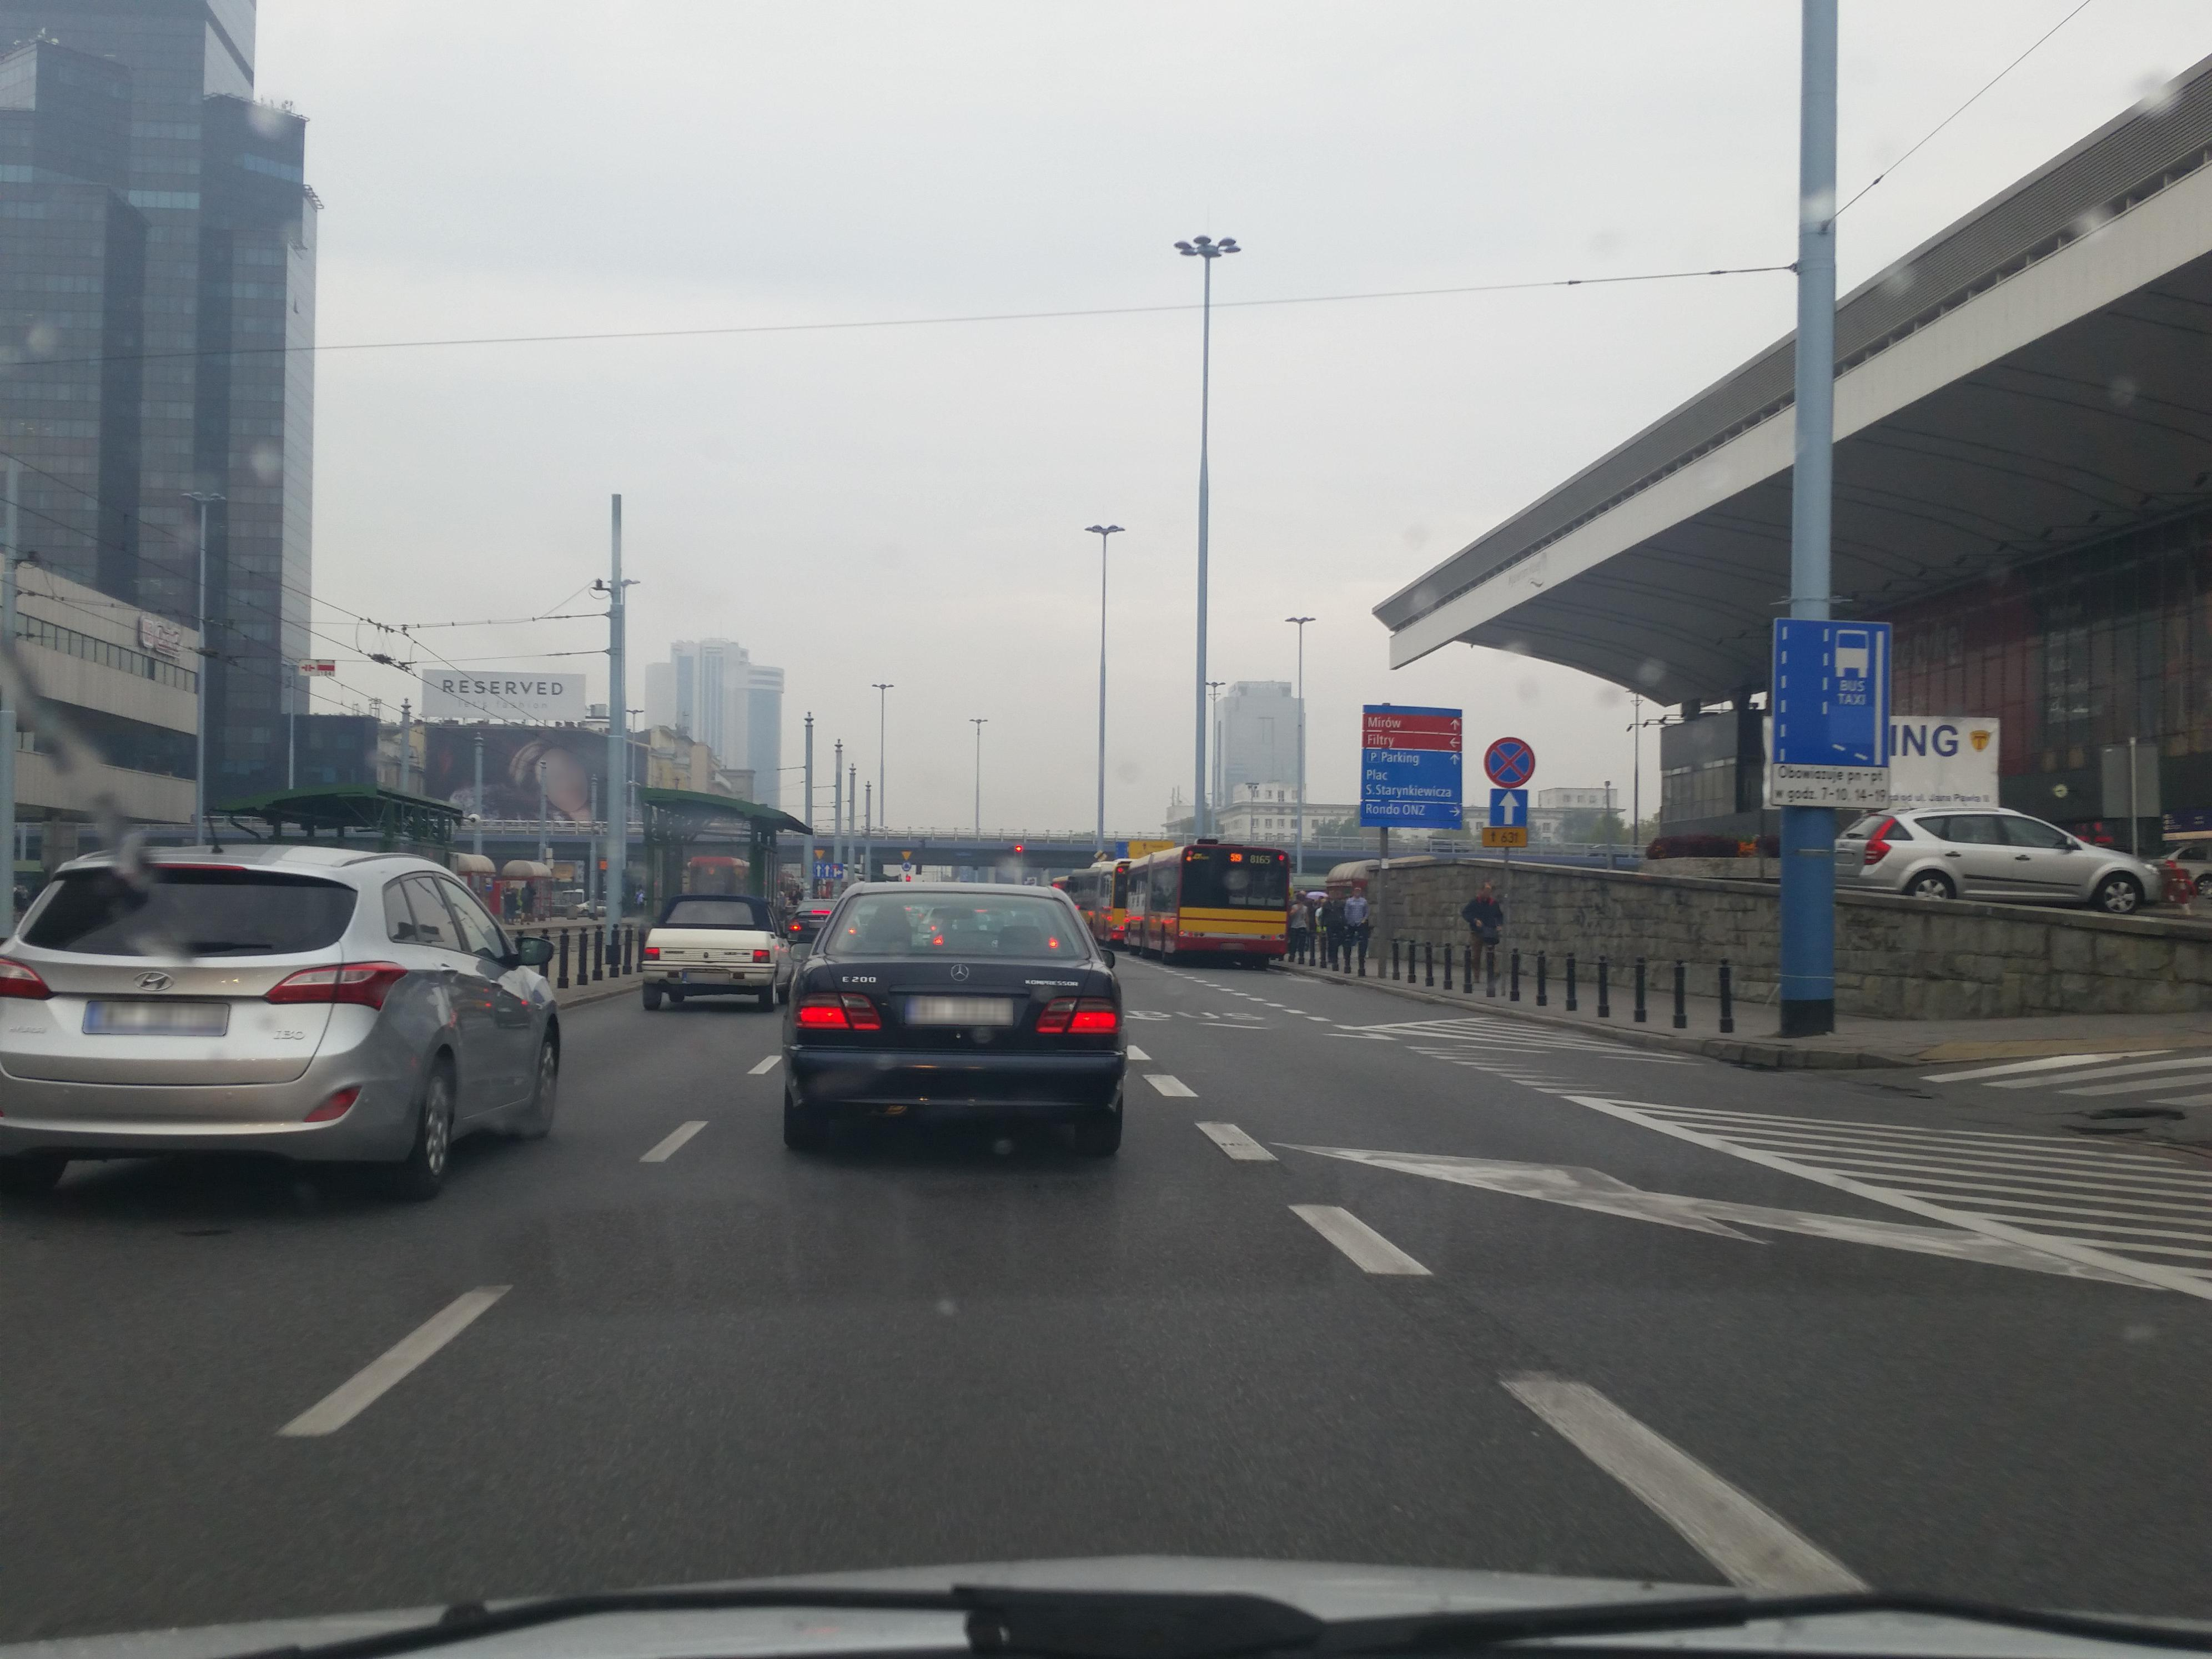
\includegraphics[width=0.20\textwidth]{train1.jpg} 
    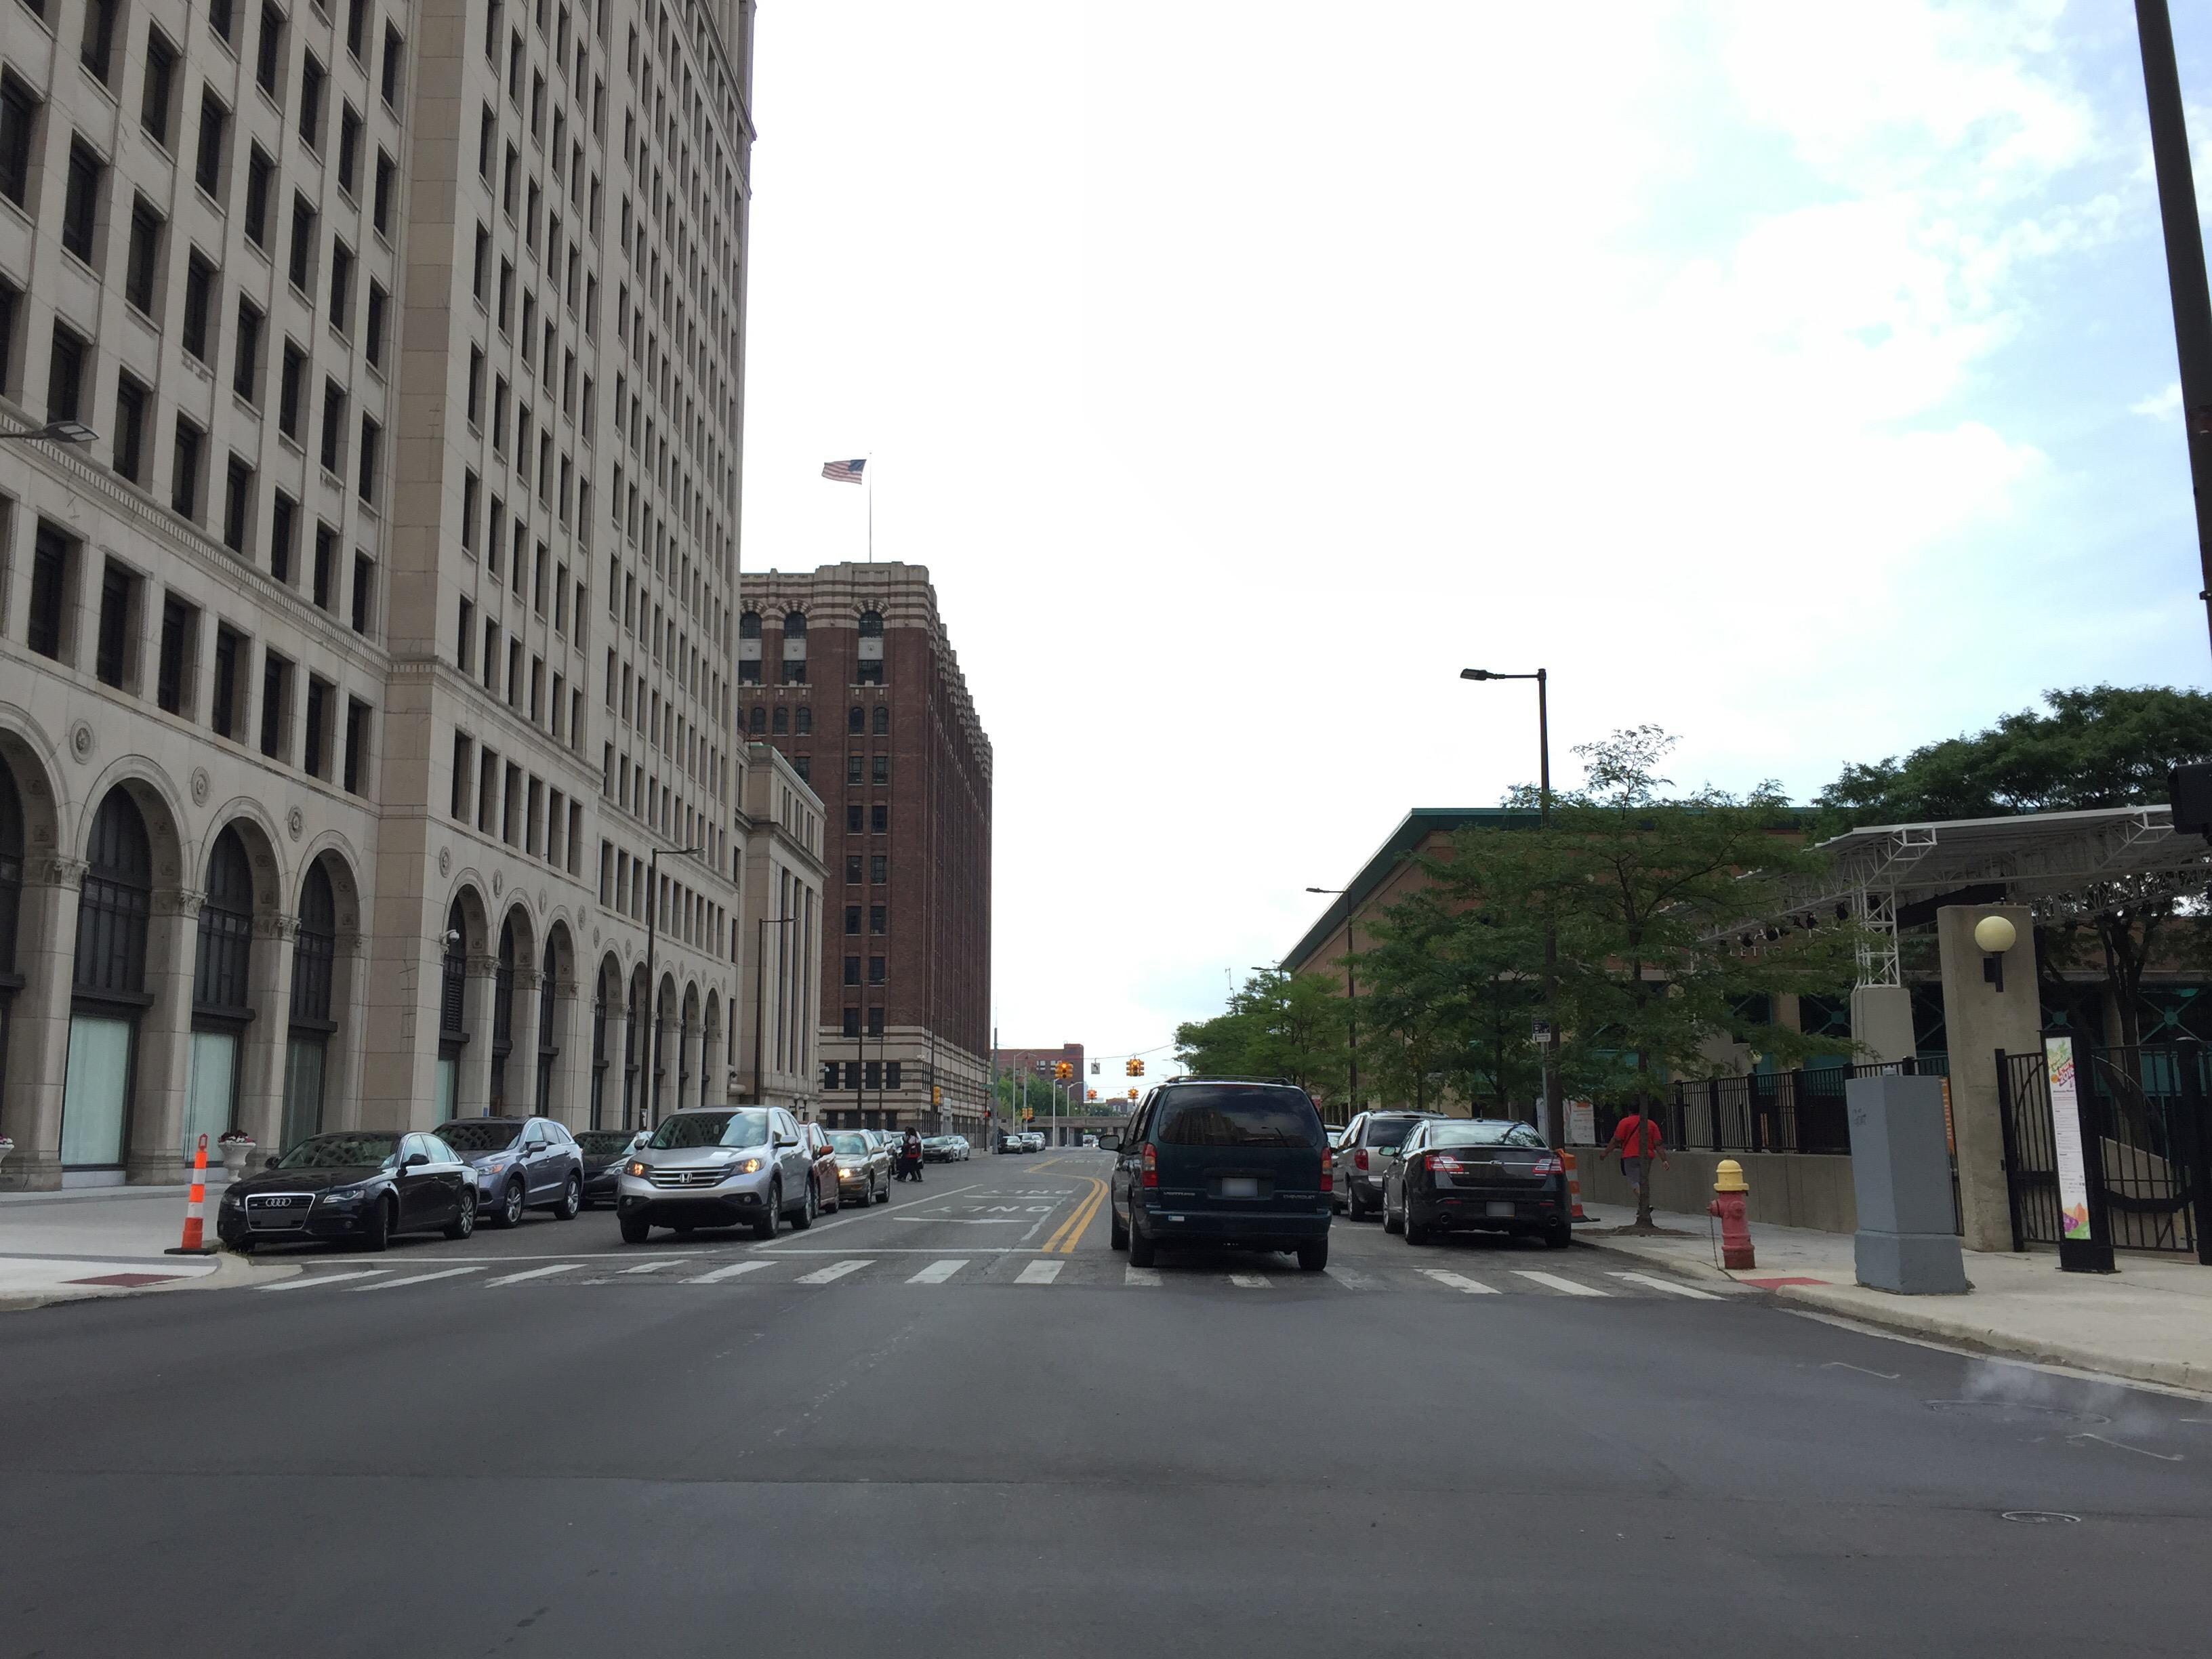
\includegraphics[width=0.20\textwidth]{train2.jpg} 
    \vspace{-2em}
\end{figure}
\begin{figure}[htbp]
    \centering
    
\includegraphics[width=0.20\textwidth]{val1.jpg} 
    
\includegraphics[width=0.20\textwidth]{val2.jpg} 
    \vspace{-2em}
\end{figure}
\begin{figure}[htbp]
    \centering
    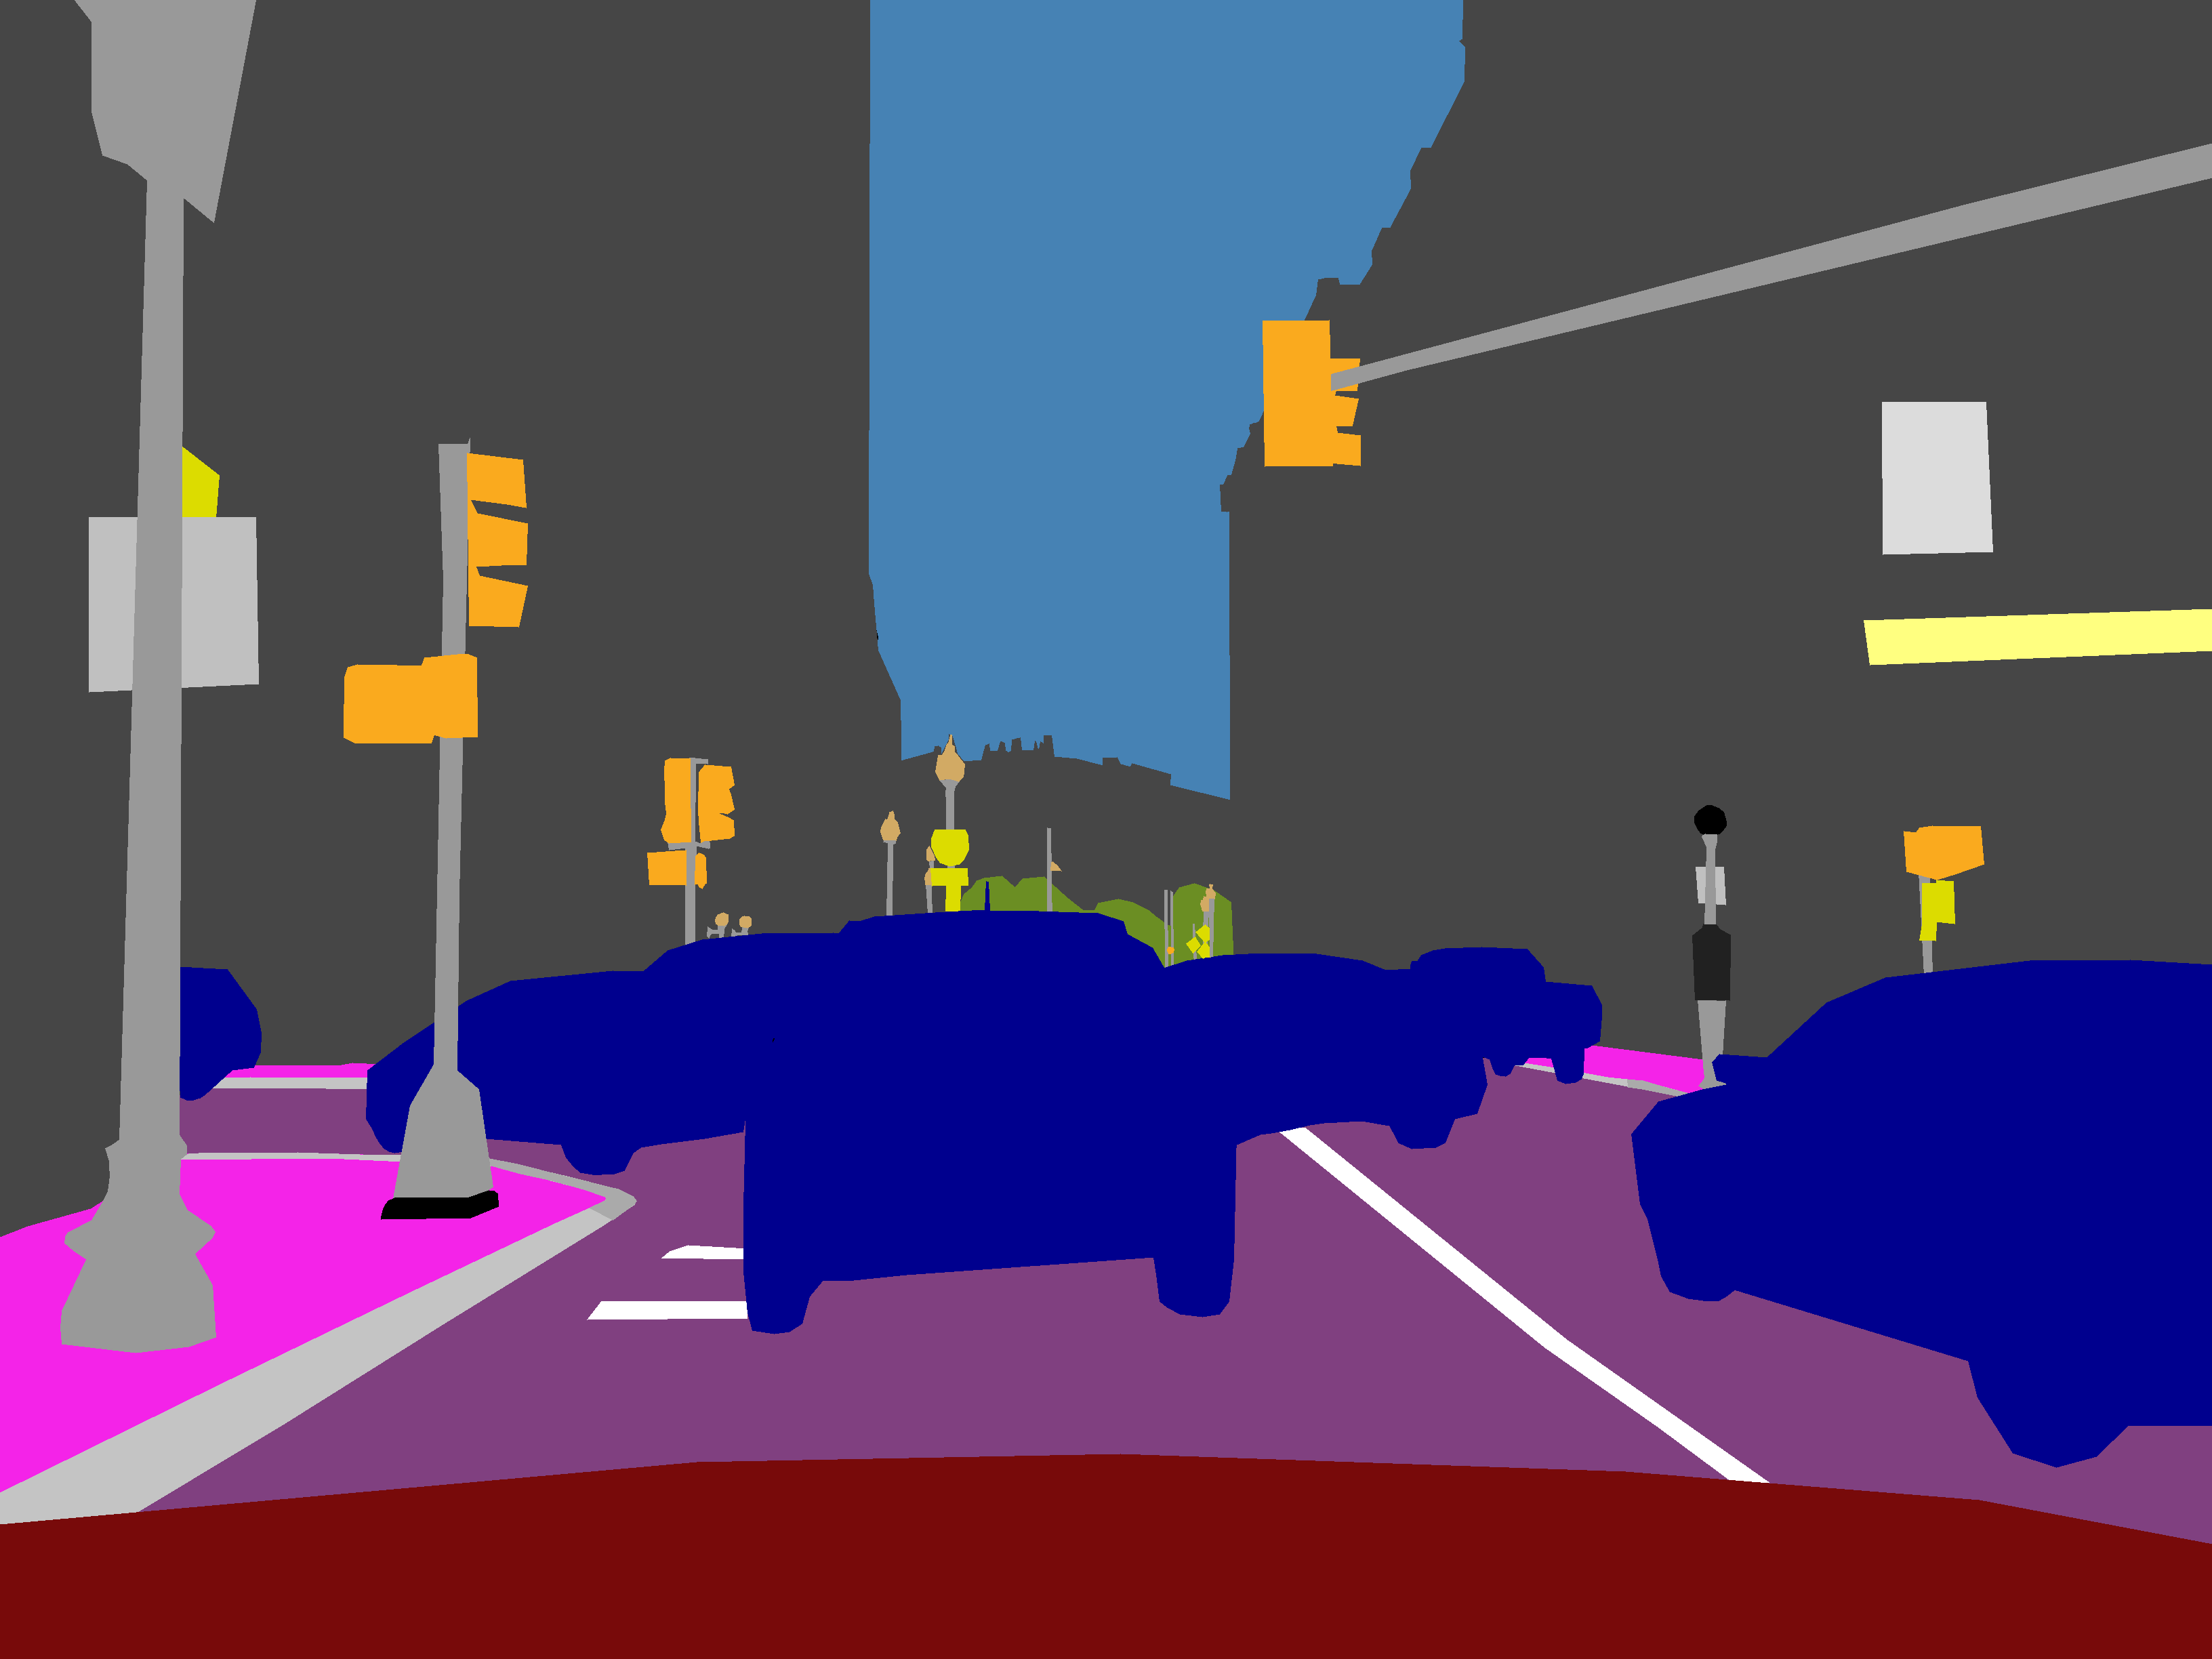
\includegraphics[width=0.20\textwidth]{labval1.jpg} 
    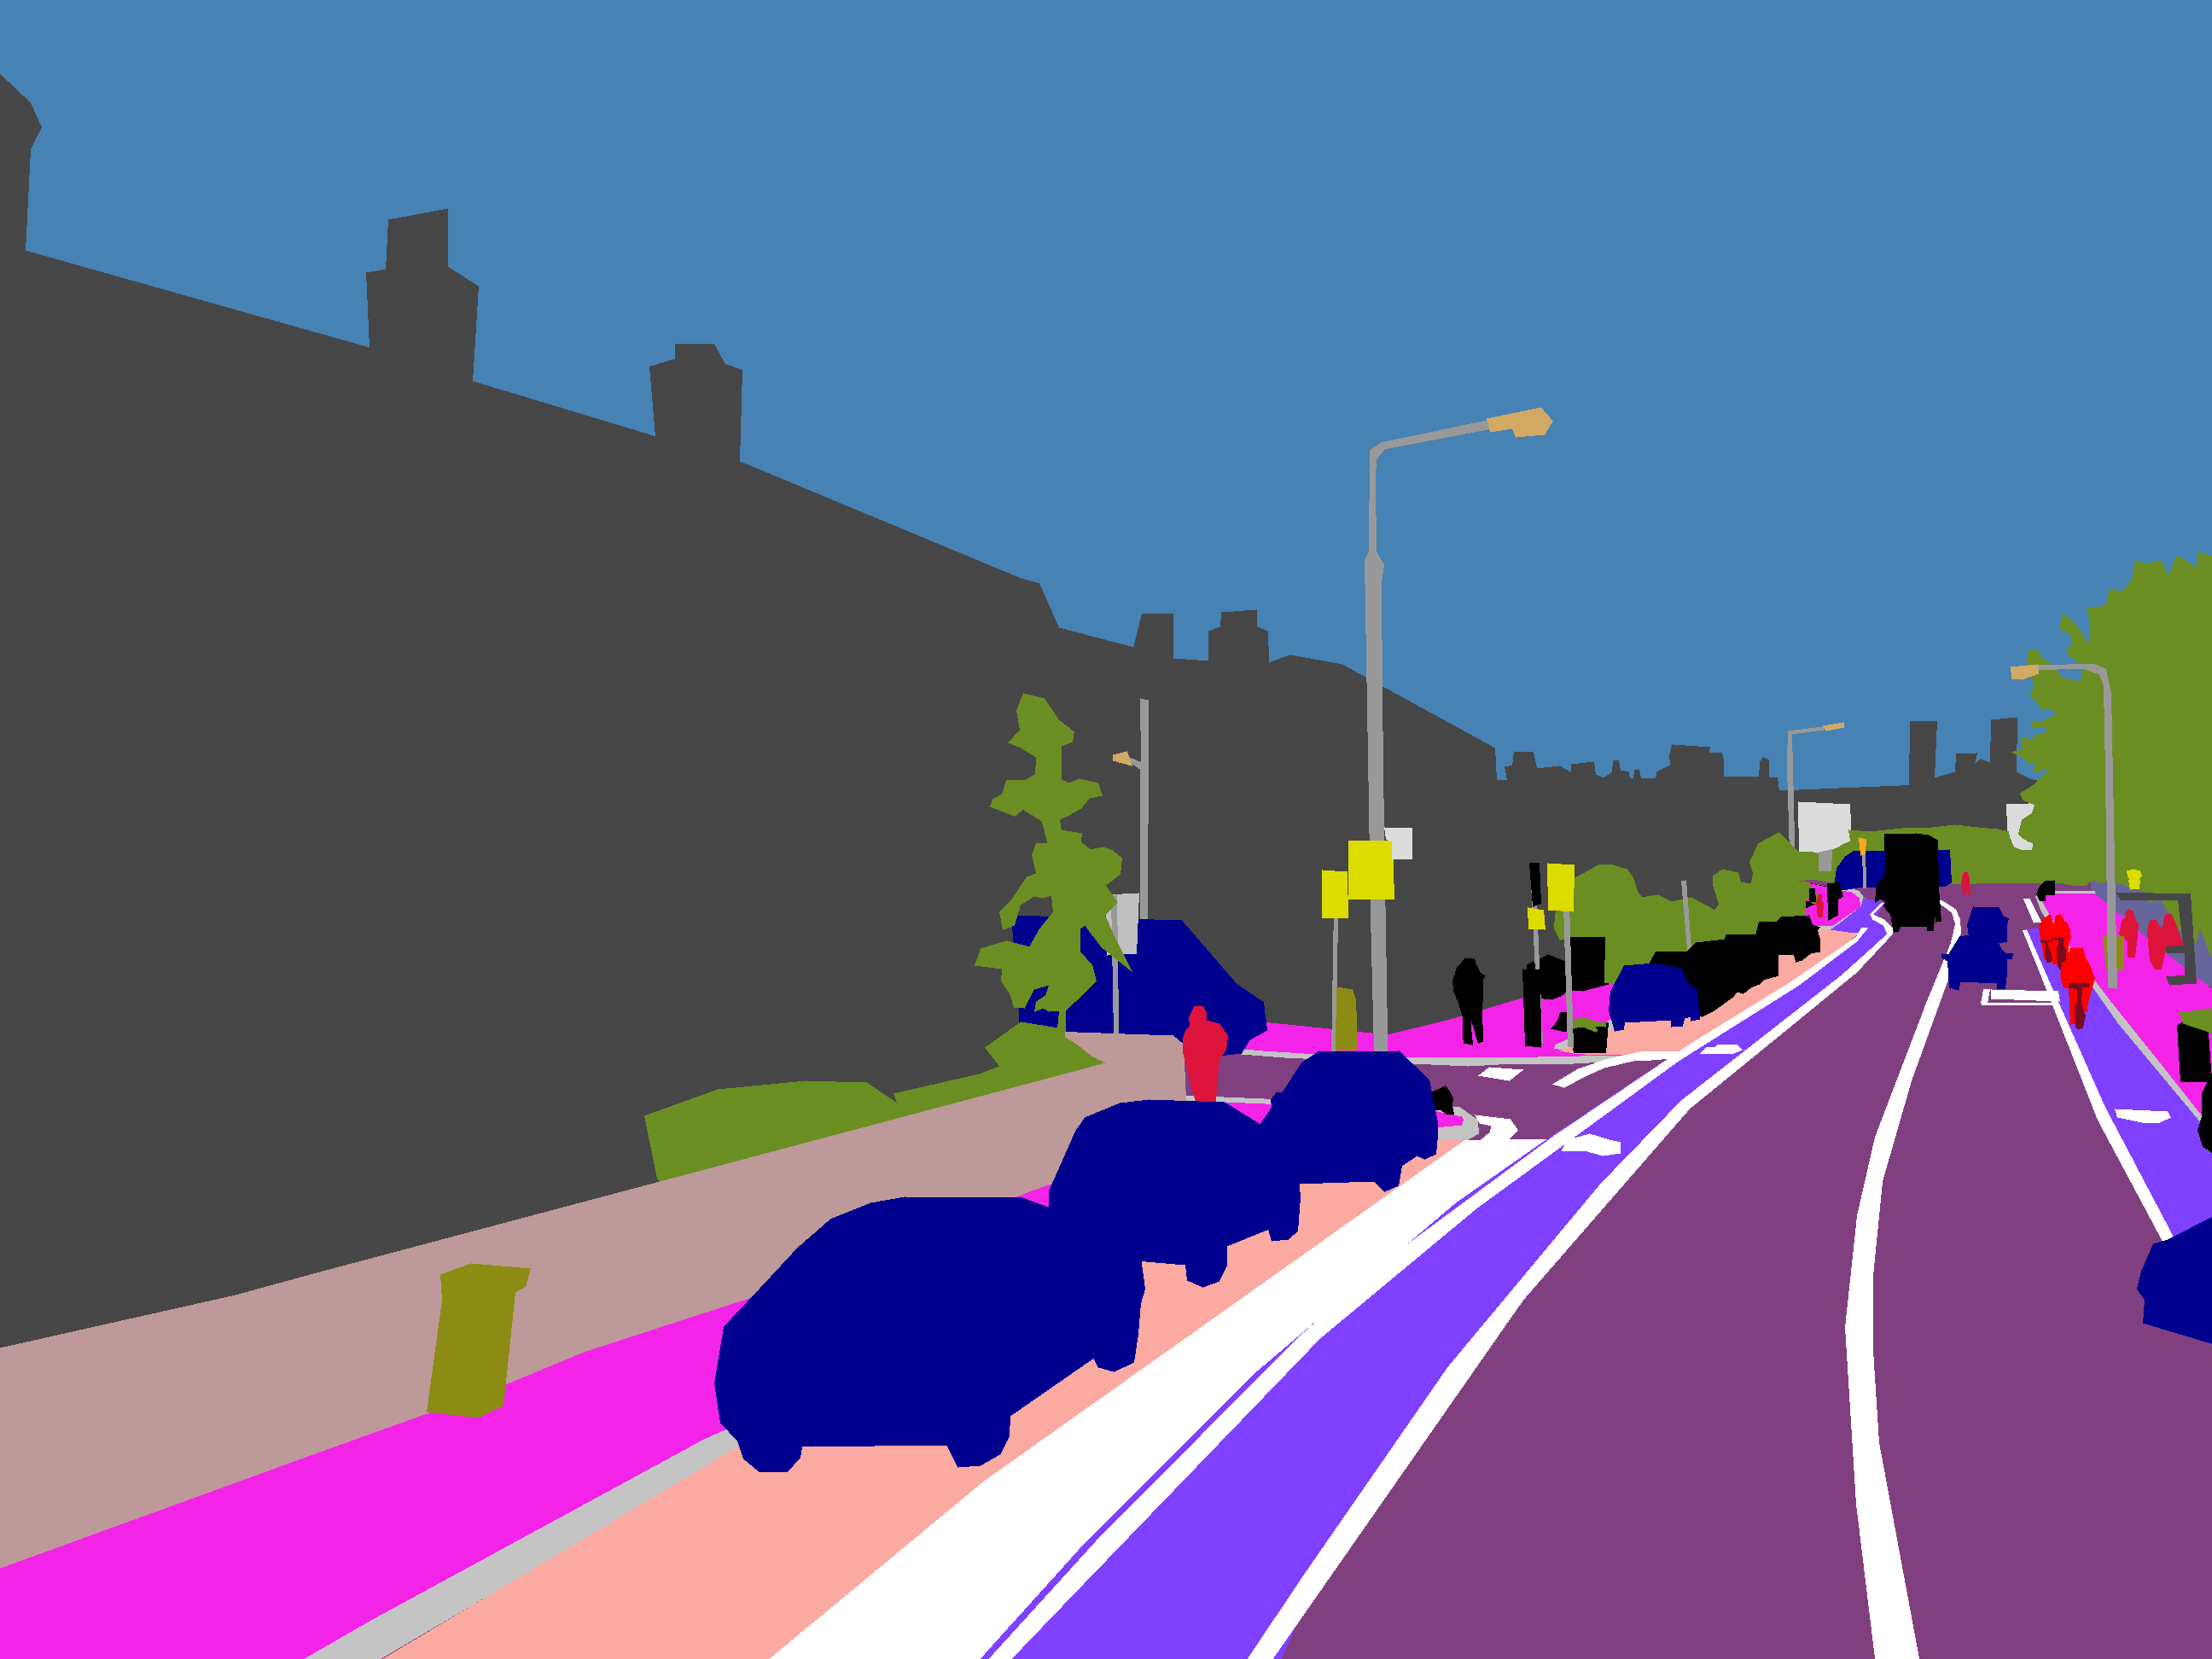
\includegraphics[width=0.20\textwidth]{labval2.jpg} 
    \caption{Glimpse of Mapillary Vistas Dataset}
    \label{fig}
\end{figure}

\section{Related work}
Instance segmentation has been one of the fast-growing topics in computer vision and we have seen several developments in the recent past. Being one of the foundational challenges in scene understanding, it focuses on detecting and outlining certain objects in the image as well as classifying each of them into a certain category. As suggested by the literature, there have been many approaches that attempt address this problem by making the methods more accurate and efficient. Some of them are:
\subsection{Mask-RCNN}
Among the most widely approaching mask R-CNN by He et al. (2017), which was developed from Faster R-CNN by adding a new branch that predicts segmentation masks alongside with the existing branch for the bounding box detection and clustering. Since then, Mask R-CNN has emerged as the start point of many instance segmentation tasks due to the high overall accuracy and its generality to different datasets. Nevertheless, it has been revealed that this approach does not perform effectively while dealing with overlapping objects and it has poor boundary accuracy despite having high accuracy in street environment such as Mapillary Vistas.
\\
\subsection{Detectron2}
The Detectron2 of Facebook's AI research once again extends Mask R-CNN while bringing several advancements in training pipelines, modularity, and scalability to handle multiple large-scale datasets. Real-time segmentation has been relevant in implementing Detectron2 across different domains such as automobile driving, medical image analysis, and robotics vision. While highly efficient, Detectron2, however, has revealed biases particularly when applied on complex scenarios to which non-vehicle objects dominate such as the street view imagery within the Mapillary Vistas.
\\
\\
In our work, we aim to build upon these existing models and frameworks by addressing the gap in detecting diverse road infrastructure elements. By evaluating state-of-the-art models like Mask R-CNN and Detectron2 on the Mapillary Vistas dataset, we aim to enhance their generalization capabilities and improve their detection of non-vehicle objects in complex, real-world street environments.

\section{Methodology}
\subsection{Background}
\subsubsection{Resnet50}
ResNet50 or Residual Network 50 is a deep neural network architecture which employs the concept if residual learning, which defined a new way of training deeper networks where the vanishing gradient proved quite challenging. It comprises 50 layers comprising of the residual blocks. The simplest one implemented in the residual blocks is the so-called shortcut connection, enabling the input to skip over some other layers and connect directly to the output. This greatly assists in terms of information retention as well as gradient flow stabilization.

ResNet50 has 5 stages and in each of them there are several convolutional layers which are grouped into residual blocks. These stages successively decrease the spatial size of the feature maps but at the same time increase depth. This indicates that despite the model being able to detect hierarchical features from simple edge detection at the first levels to object parts at deeper layers, it is well suited for the purpose of object recognition. Each residual block employs a bottleneck design consisting of three layers:

\begin{itemize}
    \item A convolution is performed to reduce the dimensionality of the matrix from 2x1 to 1x1. This one has a convolution of 3 layers by 3 layers for feature extraction.
    \item The next 1x1 convolution to bring back the appropriate dimensions.
    \item This structure contributes largely to the performance and effectiveness of ResNet50 and that makes it the most preferred when used as the base model when developing instance segmentation algorithms such as the Mask-RNN.\\
\end{itemize}
\begin{figure}[htbp]
    \centering
    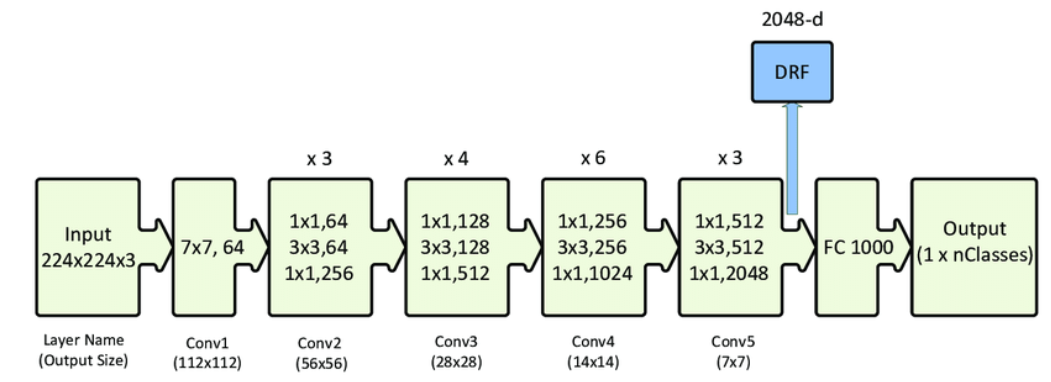
\includegraphics[width=0.45\textwidth]{resnet50.jpg} 
    \caption{Resnet50}
    \label{fig}
\end{figure}
\subsubsection{Residual Blocks}
They are the most fundamental contributions of ResNet where the output of a layer is added to the input using skip connection. This identity shortcut assists in savings an information and keeps the gradients unsubstantiated during backpropagation. It looks like there are two or three layers of convolution which are bypassed with the shortcut connection. ResNet solves the issue of gradient vanishing by adding the original input data into the output from the layers, and let the very deep models be trained, which is exactly the point that is essential to perceiving the fine-grained changes in large-scale datasets like Mapillary Vistas.
\\
For instance segmentation Mask R-CNN has used ResNet50 as the feature extractor which helps to capture low level to high level features of an image. This makes it suitable to detect complex objects on street level images with different weather conditions and geographic contexts of the images available in our dataset.
\\
\begin{figure}[htbp]
    \centering
    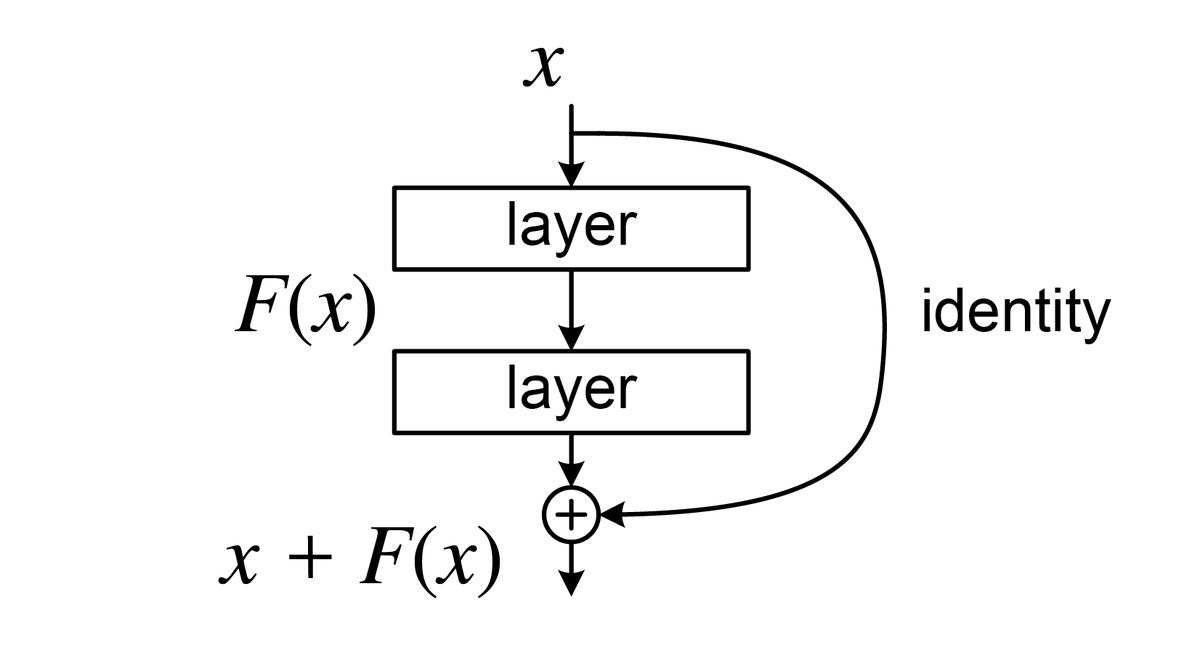
\includegraphics[width=0.40\textwidth]{ResBlock.jpg} 
    \caption{Residual Block}
    \label{fig}
\end{figure}
\subsection{Proposed Methodology}
\subsubsection{Mask-RCNN} 
Mask R-CNN is a descendant of the Faster R-CNN where an extra branch is proposed to predict segmentation masks. The model is divided into two main parts: including the backbone or the feature extractor, the neck, and the head – region proposal and mask prediction. In our case, to detect feature maps from the input images, we employ the ResNet50 model which is initially to extract images from the input. The output of the feature maps is then put through a Region Proposal Network (RPN) which proposes regions that contain objects. These proposals are then passed through the mask head which gives binary masks for each of the object instances so that our network is able to localize and segment out individual objects.

In the case of experimenting with Mask R-CNN on the Mapillary Vistas dataset, we provided details of how the model performs on complex scenes on the roads. Although Mask R-CNN gives a promising result for detecting distinct objects such as vehicles, it poorly detects smaller objects and other components of the environment that are significant for autonomous driving, for instance, road signs, lanes, and pedestrians. One of the primary challenges that we address here is how to better adjust the boundaries of overlapping objects, and how to maximize segmentation quality of objects of different shapes and sizes in the road context at that.

To deal with these issues we evaluated the idea of increasing the size of training set and adjusting the hyperparameters for better precision and less computational time. However, the identification of road infrastructure facilities such as service lanes, road markings and poles remain as some of the challenges; we hope to enhance it in next work by deploying more effective loss functions meant for boundary localization.
\\
\subsubsection{Detectron2}
The high modular and efficient Detectron2 from Facebook AI Research is an extension of the Mask R-CNN model. It offers more complex versions of various popular object detection and instance segmentation algorithms and works with Mask R-CNN, for instance. In our work, we used Detectron2 to train, using its updated procedures and the mechanisms to better work with the large datasets such as Mapillary Vistas.

Like its predecessor, the Mask R-CNN, Detectron2 relies on ResNet50 as its primary backbone but expands on the original architecture to better succeed in modern and intensive datasets. These are better data augmentation pipelines and more flexible model architectures, to make more precise predictions in less time. In our experiments, Detectron2 gives a slight edge when it comes to computational speed but manages to shave of time from the training process while still retaining comparable accuracy.

The primary benefit of utilizing Detectron2 in our project was it outperforms the handling of scale and diversified datasets like Mapillary Vistas. Nonetheless, it was also seen to detect large objects like cars easier, as was seen with Mask R-CNN and failed to locate signs and other small features like lane markings that are less conspicuous in the input frame. To this end, we rescaled Detectron2’s anchor boxes and retrained the model at a higher resolution for small objects. This led to improved recall for detecting small objects but there still is potential to fine tune the edges of the partial overlap regions.\\
\\
\\

\begin{figure}[htbp]
    \centering
    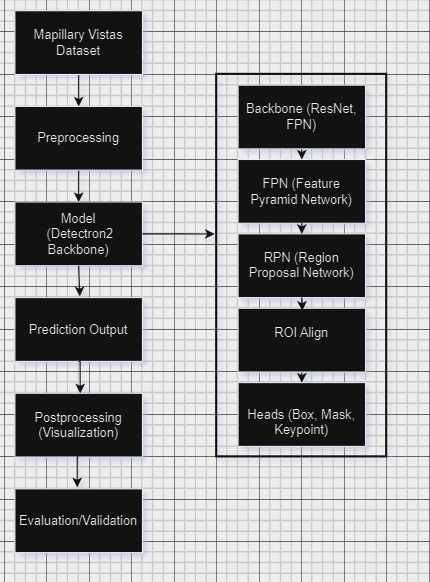
\includegraphics[width=0.40\textwidth]{projarch.jpg}
    \caption{Architecture}
    \label{fig}
\end{figure}
In figure 4, starting from the left, we started by depicting the images of the dataset, indicating its dimensions, show the dataset flow, detailing the images and their panoptic segmentation annotations.
\begin{itemize}
    \item Prepossessing: Data Augmentation, resizing or normalization
    \item Model (Detectron2 Backbone): Splitted the model into its main components like
    \\1. Backbone(ResNet, FPN)
    \\In real image input the first convolution layer, then through the batch norm and followed by a ReLU activation.\\
    ResNet Stages (Stage 1, 2, 3, 4): Subsequently the image goes through several residual blocks (ordinarily four stages of ResNet) to capture varying levels of features. These residual blocks proposed are made up of the convolutional layers and skip connections. The size of the feature maps decreases as the depth increases. These deeper layers (e.g., Res4, Res5) get higher level of features.\\
    FPN: After getting feature maps of ResNet, the Feature Pyramid Network (FPN) fusion is performed on symbol maps of multiple scales from various ResNet stages.\\
    Top-down and lateral connections: FPN combines top-down and lateral connections to improve the multi-scale feature maps. One of the pathways is top down, which actually scales up the higher-level or more abstract feature maps from deeper layers and they are combining with he lower-level or higher resolution feature maps through a process called lateral connection. This results in a feature pyramid where abundant and detailed feature information at different scales can be obtained for both small and large sized objects.

    2. RPN (Reigon Proposal Network): To generate potential object proposols, outputs bounding box coordinates and objectness scores.

    3. ROI align and Heads (Box, Mask, Keypoint)\\
    \item Prediction Outputs: we show the output flow, leading to predicted instance masks, labels, and confidence scores.
    \item Postprocessing (Visualization): Rendering of Instance Masks overlaid on original mask
    \item Evaluation/Validation (COCO Metrics): IoU (Intersection over Union) and mAP (mean average precision) 
\end{itemize}

Input Image → ResNet (Conv1, Res2, Res3, Res4, Res5) → FPN (P2, P3, P4, P5) → RPN → ROI Align → Box Head / Mask Head → Outputs (masks, boxes, etc.)


\section{Experiments}
In this section, we'll be describing the methodology to compare the performance of the Mask R-CNN and Detectron2 on the custom subset of Mapillary Vistas. The main goal of these experiments is to evaluate and compare the performance of these high-performing grids in terms of accuracy, time and boundary detection on instance segmentation in complex road scenes.
\subsection{Dataset}
3,700 images were selected from the Mapillary Vistas dataset for using them in the training, validation, and testing of the model. These images include multiple scenarios that can be met on the streets in different geographical areas, at different times of the day/night and in different climates. Every picture is marked with object masks for dozens of object categories, with a particular emphasis on recognizing elements of road infrastructure such as cars, pedestrians, and signs.
\begin{itemize}
    \item Training set: 2700 images
    \item Validation set: 700 images
    \item Testing set: 500 images
\end{itemize}
The annotations are of both bounding boxes and segmentation masks, which enables one to compare and contrast the results of an algorithm in detecting objects and segmenting the instances out of the objects.For the experiments, all the images were resized to 256x256 pixels and the dataset was split into 13 different road facility classes.

\subsection{Evaluation Metrics}
In addition to that accuracy, precision, recall, F1-score and memory were used as some standard parameters to assess performance. The efficiency of the models was evaluated using the following:
\begin{itemize}
    \item Mean Average Precision (mAP): On the basis of Intersection over Union (IoU) values – IoU= 0.5, IoU = 0.75 and IoU= 0.95.
    \item Boundary Precision: Quantitatively measures the difference between the predicted object boundaries and actual boundaries, paying attention to the issues of small object and overlapping instances.
    \item Inference Time: The efficiency of the computation is evaluated based on average inference time per image and inference time on both GPU and CPU.
\end{itemize}

\subsection{Training Parameters}
Our both of the models were trained using the following parameters:\\

\begin{table}[htbp]
    \centering
    \caption{Comparison of Mask-RCNN and Detectron2 Configurations}
    \label{table}
    \begin{tabular}{|p{2cm}|p{2.4cm}|p{2.9cm}|}
    \hline
    \textbf{Configuration}&\textbf{Mask-RCNN}&\textbf{Detectron (Detectron2)}\\
    \hline
    \textbf{Optimizer} & SGD with Momentum(0.9) & SGD with Momentum(0.9)\\
    \hline
    \textbf{Learning Rate} & start with 0.001, with a step-wise decay by a factor of 10 at 5,000 and 8,000 iterations & 0.00025 warm-up for 1,000 iterations\\ 
    \hline
    \textbf{Batch Size} & 4 images & 2 images\\
    \hline
    \textbf{No. of Epochs} & 10 Epochs & 1,000 iterations\\
    \hline
    \textbf{Loss Function} & Classification Loss, Bounding box regression loss, equally weighted & same as Mask-RCNN\\
    \hline
    \textbf{Model Backbone} & ResNet-50 with FPN & Mask-RCNN with ResNet-50 FPN backbone\\
    \hline
    \textbf{Data Augmentation} & Images resized to 256x256 for train and validation & same as Mask-RCNN \\
    \hline
    \end{tabular}
\end{table}


\section{Results}
In this section, we show how well the proposed road facility detection models perform, those that were trained on the transferred Mapillary dataset as outlined above in this paper. 

\subsection{Evaluation Metrics}
\subsubsection{Accuracy and mAP performance}
The mAP results at different IoU thresholds: 0.50, 0.75 and 0.95 are given in table below in Table 1. Detecron2 was faster yet had a slightly higher precision compared to the Mask R-CNN model in all the listed IoU thresholds with a variation marked higher at the stricter IoU = 0.95.

\begin{table}[htbp]
    \centering
    \caption{Accuracy and mAP performance}
    \label{table}
    \begin{tabular}{|c|c|c|c|}
    \hline
    \textbf{model}&\textbf{mAP (IoU=0.50)}&\textbf{mAP (IoU=0.75)}&\textbf{mAP (IoU=0.95)}\\
    \hline
    Mask-RCNN & 71.2\% & 55.4\% & 42.8\%\\
    \hline
    Detectron2 & 73.9\% & 58.1\% & 45.6\%\\
    \hline
    \end{tabular}
\end{table}
The high effectiveness of Detectron2 is greatly enhanced through the new feature pyramid network and the region proposal system that allow handling small objects much more effectively and intricate occlusions within urban environments.\\

\subsubsection{Boundary Precision}
One of the significant goals of the experiments was to evaluate the efficacy of models in improving boundary recall of detected objects, especially with conditions of overlapping items and occlusions. As far as boundary accuracy goes, Mask R-CNN performed significantly better compared to others, especially for small objects like traffic signs and poles, with a boundary precision of 62.5\% compared with Detectron2's 60.3\%.\\

\subsubsection{Inference Time}
Given that instance segmentation will be implemented in real time, particularly in areas such as autonomous driving, computational efficiency becomes a priority. We evaluated the inference time per image across the various GPU and CPU configurations.\\
\begin{table}[htbp]
    \centering
    \caption{Comparison of Inference Times}
    \label{table}
    \begin{tabular}{|c|c|c|}
    \hline
    \textbf{model}&\textbf{Inference Time (GPU)}&\textbf{Inference Time (CPU)}\\
    \hline
    Mask-RCNN & 0.32 secs & 3.89secs\\
    \hline
    Detectron2 & 0.28 secs & 3.65 secs\\
    \hline
    \end{tabular}
\end{table}
\\Detectron2 demonstrated enhanced inference speed on both GPU and CPU platforms, rendering it more appropriate for applications requiring real-time processing. Nonetheless, the variance in inference duration's was comparatively minor, and the decision between the two models may hinge on the particular trade-offs associated with accuracy and computational expense.\\

\subsubsection{Model Robustness}
Both models were assessed regarding their capacity to generalize across varying weather conditions and geographic contexts. Detectron2 demonstrated superior resilience in managing unfavorable weather scenarios, including rain and fog, where occlusions were more common. Conversely, Mask R-CNN showed a greater proficiency in identifying small objects within densely populated urban environments.

\subsection{Image comparison Results}
After calculating all the metrics, we have validated the trained models on our custom mapillary dataset. Down below are some results generated by our models:\\

\begin{figure}[htbp]
    \centering
    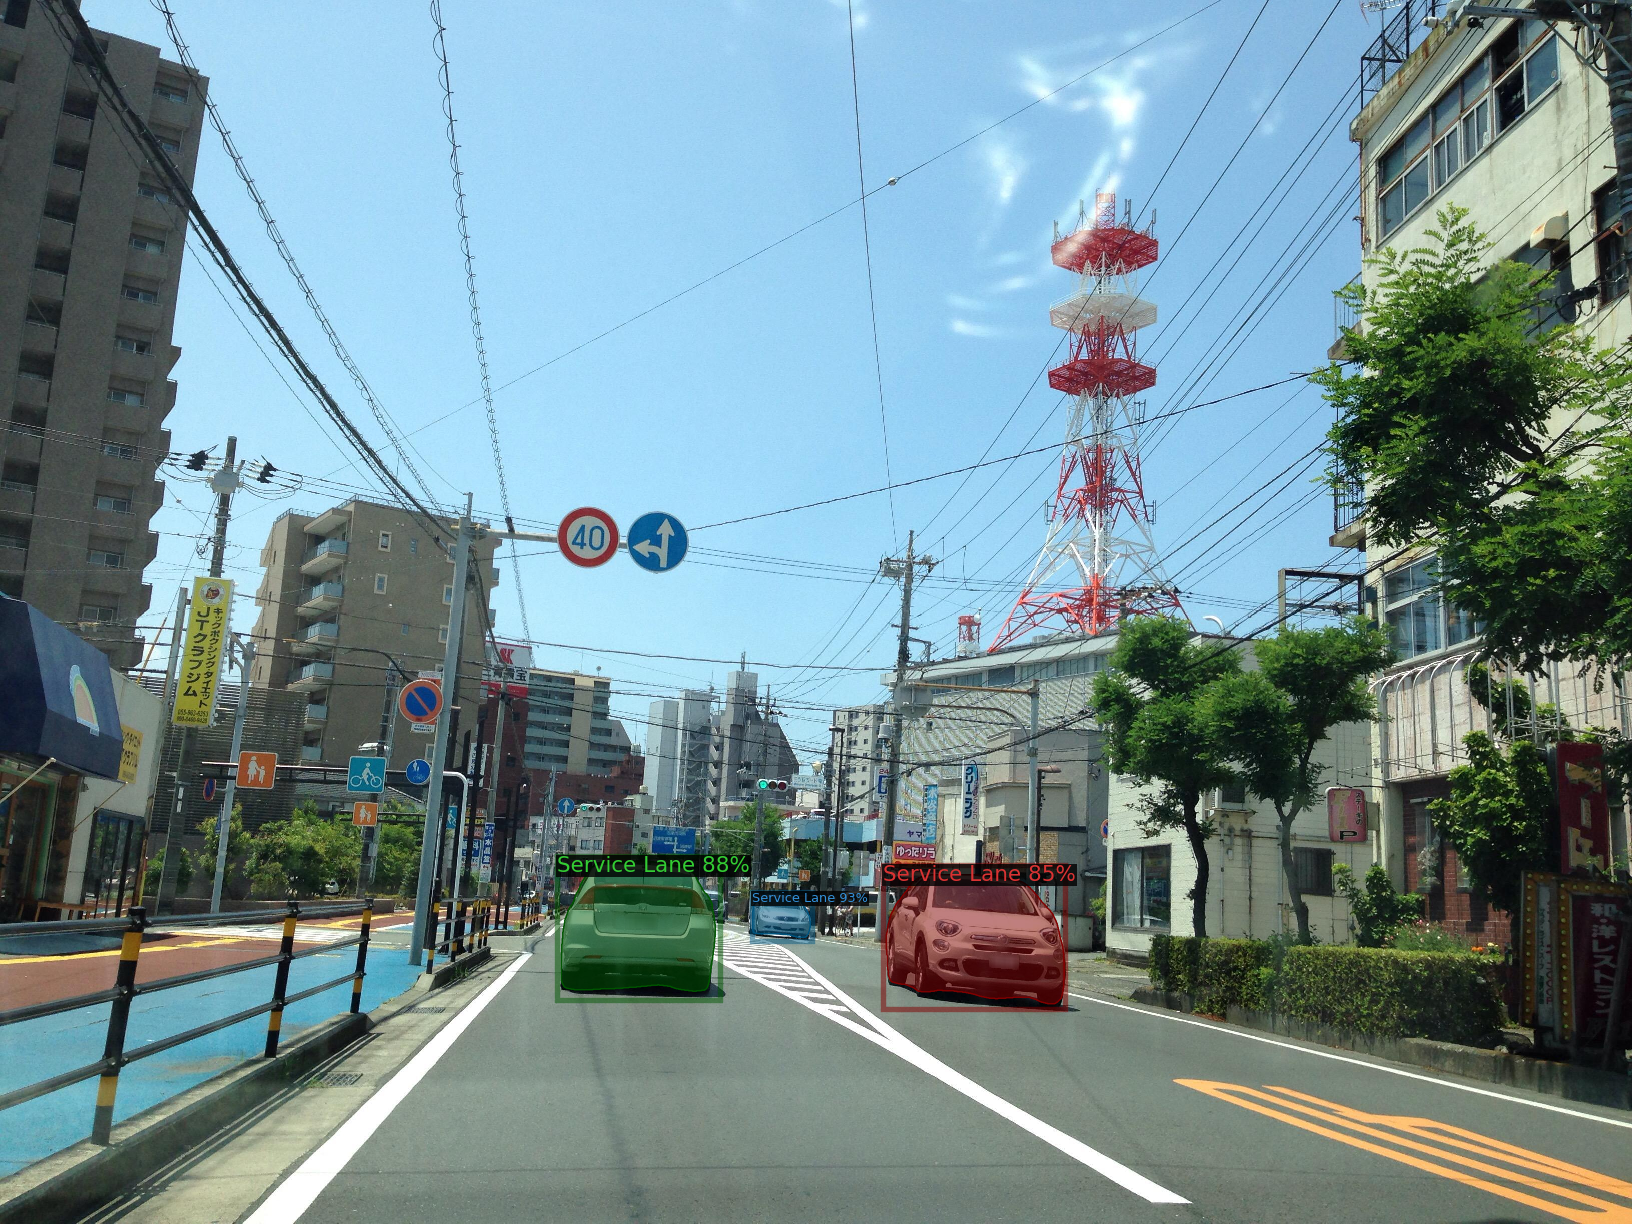
\includegraphics[width=0.24\textwidth]{detectres2.png} 
    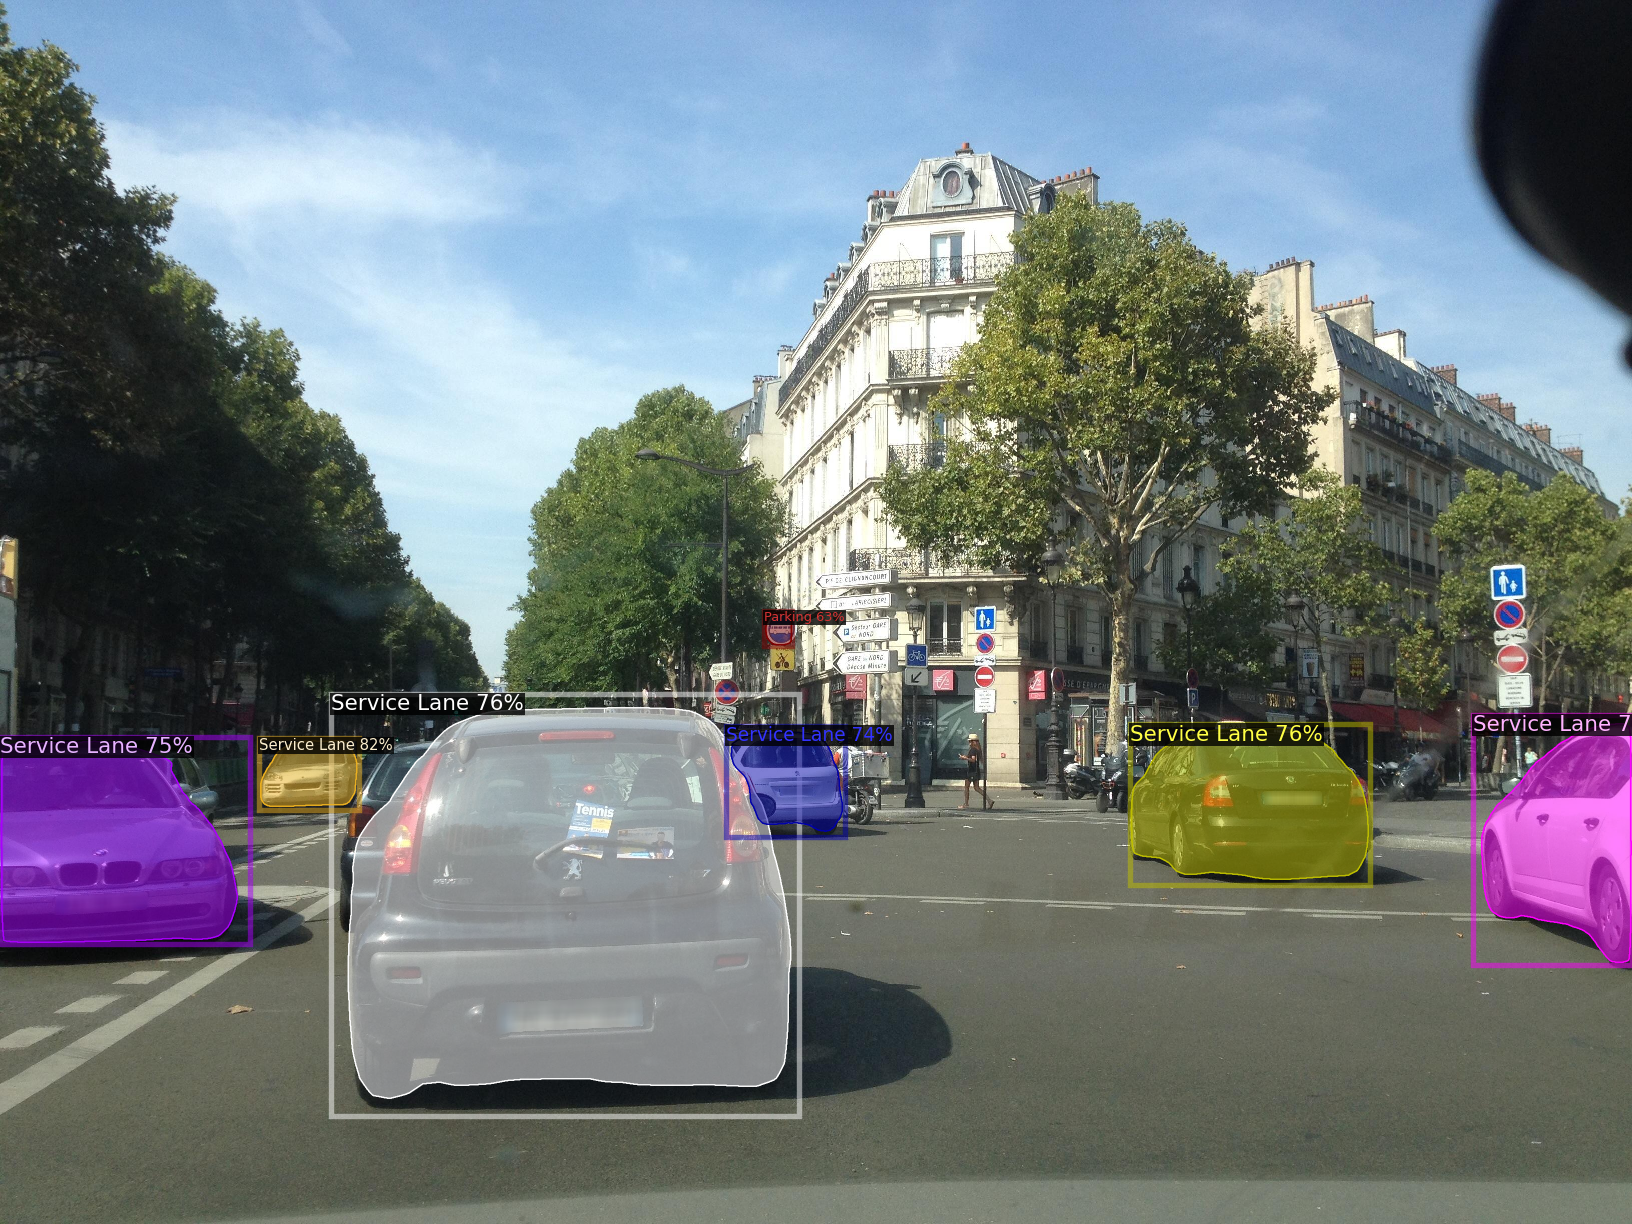
\includegraphics[width=0.24\textwidth]{detectres1.png}
    \caption{(a)Detectron Model}
    \label{fig}
    \vspace{-2em}
\end{figure}
\begin{figure}[htbp]
    \centering
    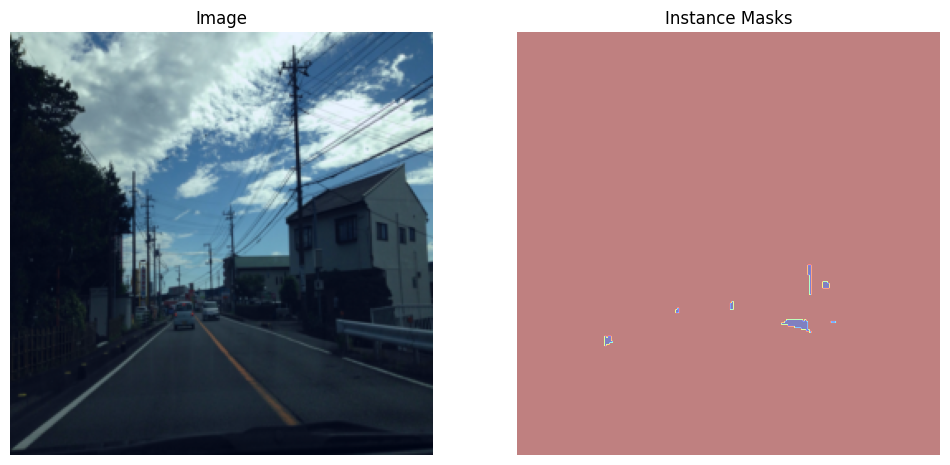
\includegraphics[width=0.50\textwidth]{mask.png} 
    \caption{(a)Mask-RCNN Model}
    \label{fig}
\end{figure}
\section{Conclusion}
In this paper, a comparative evaluation of two advanced deep learning architectures, specifically Mask R-CNN and Detectron2, in the case of instance segmentation for the detection of road facilities has been made. Based on a subset derived from Mapillary Vistas, our results indicated that both models accurately detected major road facilities and infrastructure with remarkable performance both on the validation set and the test set.

Mask R-CNN, with a ResNet-50 acting as its backbone and Feature Pyramid Network(FPN), was good at detecting bigger objects such as cars and poles but faced some challenges with smaller objects like those of traffic signs. Conversely, Detectron2, using the same backbone, showed faster inference timings with fewer computational costs; it, therefore, proved to be a better choice when speed becomes a concern. The two models generalized robustly to the different scenarios of urban and rural environments since supported by the results in the varied images in the dataset.

The results show that both models are effective for detecting road facilities, where trade-offs between detection accuracy and computational efficiency have to be taken into account. Mask R-CNN shows robustness in tasks requiring high precision, particularly on larger objects. For applications that require faster inference and also reduced resource usage, a viable alternative at close to the same accuracy is Detectron2.

Future work will study other models, like YOLOv7\cite{1}-\cite{10}, which can possibly  improve the detector of small objects and train models of complexes augmentation techniques. The outcome in this paper adds to an increasingly body of knowledge regarding instance segmentation for road facility detection, which guides model selection in intelligent transportation systems and the construction of HD maps.

\begin{thebibliography}{00}
\bibitem{1}Z. Yang, C. Zhao, H. Maeda, and Y. Sekimoto, “Development of a Large-Scale Roadside Facility Detection Model Based on the Mapillary Dataset,” Sensors, vol. 22, no. 24, p. 9992, Dec. 2022
\bibitem{2}A. M. Hafiz and G. M. Bhat, “A survey on instance segmentation: state of the art,” International Journal of Multimedia Information Retrieval, vol. 9, no. 3, pp. 171–189, Jul. 2020
\bibitem{3}G. Neuhold, T. Ollmann, S. Bulò, P. Kontschieder, and M. Research, “The Mapillary Vistas Dataset for Semantic Understanding of Street Scenes.” 
\bibitem{4}R. Mohan and A. Valada, “EfficientPS: Efficient Panoptic Segmentation,” arXiv.org, Feb. 01, 2021.
\bibitem{5}C. Fan et al., “DiverGen: Improving Instance Segmentation by Learning Wider Data Distribution with More Diverse Generative Data,” arXiv.org, 2024.
\bibitem{6}X. Wang, T. Kong, C. Shen, Y. Jiang, and L. Li, “SOLO: Segmenting Objects by Locations,” arXiv (Cornell University), Dec. 2019.
\bibitem{7}L. Chen, Y. Fu, K. Wei, D. Zheng, and F. Heide, “Instance Segmentation in the Dark,” International Journal of Computer Vision, vol. 131, no. 8, pp. 2198–2218, May 2023.
\bibitem{8}K. He, G. Gkioxari, P. Dollár, and R. Girshick, “Mask R-CNN,” arXiv.org, 2017. 
‌\bibitem{9}“Path Aggregation Network for Instance Segmentation,” ieeexplore.ieee.org.
‌\bibitem{10}[1]L. Yang, N. Xu, and A. Research, “Video Instance Segmentation.” 
‌‌
\end{thebibliography}

\end{document}
